% ARPEGOS:  Automatized Roleplaying-game Profile Extensible Generator Ontology based System %
% Author : Alejandro Muñoz Del Álamo %
% Copyright 2019 %

% Section 5.1: Arquitectura del Sistema
\section{Arquitectura del Sistema}
Esta sección tratará de describir la arquitectura física y lógica del sistema. Para ello se abordará cómo 
está estructurado, su funcionamiento y la forma de interactuar entre los diferentes componentes del 
proyecto.

\subsection{Arquitectura Física}
El apartado de arquitectura física del sistema hace referencia a los componentes, tanto hardware como software,
necesarios para poder lanzar la aplicación resultante del proyecto. Este proyecto no está únicamente orientado 
a los usuarios de la aplicación, sino que también está orientado a los desarrolladores de \textit{RPGs}, dándoles acceso
a una herramienta que sólo requiere la elaboración del fichero de información del juego, reduciendo los tiempos de 
producción del generador de personajes, de manera que los usuarios puedan disfrutar lo antes posible de un generador 
de personajes para un juego parcial o totalmente desconocido, lo que hace a su vez que la curva de aprendizaje para 
crear personajes de ese juego se reduzca considerablemente.

\subsubsection{Requisitos para usuarios}
El único requerimiento de esta aplicación es disponer de un dispositivo móvil que tenga 
\textit{Android 9.0 (\textbf{Pie})} o superior como sistema operativo.
\textit{\textbf{No se requiere conexión a Internet para acceder a la aplicación}}. 

\subsubsection{Requisitos para desarrolladores}
En lo referente a desarrolladores de \textit{RPGs}, es necesario tener instalado \textit{\textbf{Protégé}} o una aplicación
similar para poder crear la ontología del juego que deseen introducir en la aplicación. En caso de utilizar la versión de 
escritorio de \protege, indicar que requiere al menos una versión de \textit{\textbf{Java Runtime Environment}}.

\subsection{Arquitectura Lógica}
En el apartado \ref{Arquitectura} el equipo de desarrollo indicó que ha tomado como método para elaborar la estructura del 
sistema el patrón \textit{\textbf{MVVM}}. Este patrón de arquitectura de software permite diferenciar claramente 
la lógica de una aplicación de su interfaz de usuario, lo que facilita el desarrollo, la elaboración de pruebas y la 
mantenibilidad del sistema, además de la reutilización del código y la colaboración entre desarrolladores y diseñadores
\autocite{MicrosoftMVVM}. \medskip

\subsubsection{Ventajas}
Las ventajas de utilizar el patrón \textit{MVVM} (Figura \ref*{Estructura_mvvm}) son las siguientes:
\begin{itemize}
    \item El modelo de vista permite que no sea necesario realizar ediciones masivas del código del modelo.
    \item Se pueden realizar pruebas para los modelos y los modelos de vista independientes a la vista.
    \item Las vistas pueden rediseñarse sin modificar la lógica de negocio de la aplicación.
    \item Permite independencia entre desarrolladores y diseñadores.
\end{itemize}

\subsubsection{Elementos}
\begin{figure}[H]
	\centering
	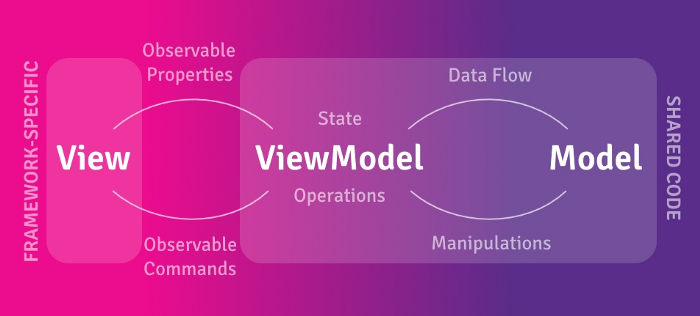
\includegraphics[scale=0.3]{Figures/mvvm_flow.png}
	\caption{Estructura del patrón \textit{MVVM}. Extraído de \textit{medium.com} \autocite*{MvvmFlowDiagram}}
	\label{Estructura_mvvm}
\end{figure}

\textit{MVVM} divide la estructura de un sistema software en tres tipos de elementos básicos, explicados de manera 
sencilla por Lou \autocite*{Lou2016}:
\begin{itemize}

    \item \textit{\textbf{Modelo}}: El modelo contiene los datos y estados de la aplicación, ya sean elementos 
    simples o clases con estructuras complejas. Puede ser que no contenga la información de manera directa, pero 
    que pueda recuperarla de manera remota. 

    \item \textit{\textbf{Modelo de vista}}: El modelo de vista tiene como objetivo dirigir los diferentes 
    estados de la vista, ya sea mediante el envío de operaciones y/o datos, o bien gestionando la lógica de la 
    vista y su comportamiento.
    
    \item \textit{\textbf{Vista}}: El componente de vista muestra la interfaz de la 
    aplicación, cuyo desarrollo está orientado más orientado a diseñadores que a programadores.

\end{itemize}
